\documentclass[12pt]{article}
\usepackage[paperwidth=16.5cm, paperheight=16.5cm, margin=0.2cm]{geometry}
\usepackage{tikz}
\usetikzlibrary{positioning, arrows.meta, calc, decorations.pathreplacing}
\pagestyle{empty}
\setlength{\parindent}{0pt}

% ============================================================================
% COLORES Y ESTILOS
% ============================================================================
\definecolor{pastelblue}{RGB}{230, 242, 252}

\tikzset{
  box/.style={
    draw, thick, fill=pastelblue,
    minimum height=1.5cm,
    minimum width=2cm,
    font=\small\sffamily,
    align=center
  },
  ffbox/.style={
    draw, thick, fill=pastelblue,
    minimum width=3.6cm, 
    minimum height=2cm,
    font=\small\sffamily,
    align=center
  },
  signal/.style={-{Stealth[length=2mm]}, thick, black}, 
  wirelabel/.style={font=\tiny\sffamily, text=black, midway, above}
}

% MUX 3-a-1
\newcommand{\drawmuxthree}[4]{
  \draw[thick, fill=pastelblue] (#1-0.4,#2+1.0) -- (#1+0.4,#2+0.6) -- (#1+0.4,#2-0.6) -- (#1-0.4,#2-1.0) -- cycle;
  \node[font=\tiny\sffamily] at (#1-0.15, #2+0.6) {00};
  \node[font=\tiny\sffamily] at (#1-0.15, #2) {01};
  \node[font=\tiny\sffamily] at (#1-0.15, #2-0.6) {10};
  \coordinate (#3_in0) at (#1-0.4, #2+0.6);
  \coordinate (#3_in1) at (#1-0.4, #2);
  \coordinate (#3_in2) at (#1-0.4, #2-0.6);
  \coordinate (#3_out) at (#1+0.4, #2);
  \coordinate (#3_sel) at (#1, #2+0.8);
}

\begin{document}
\noindent
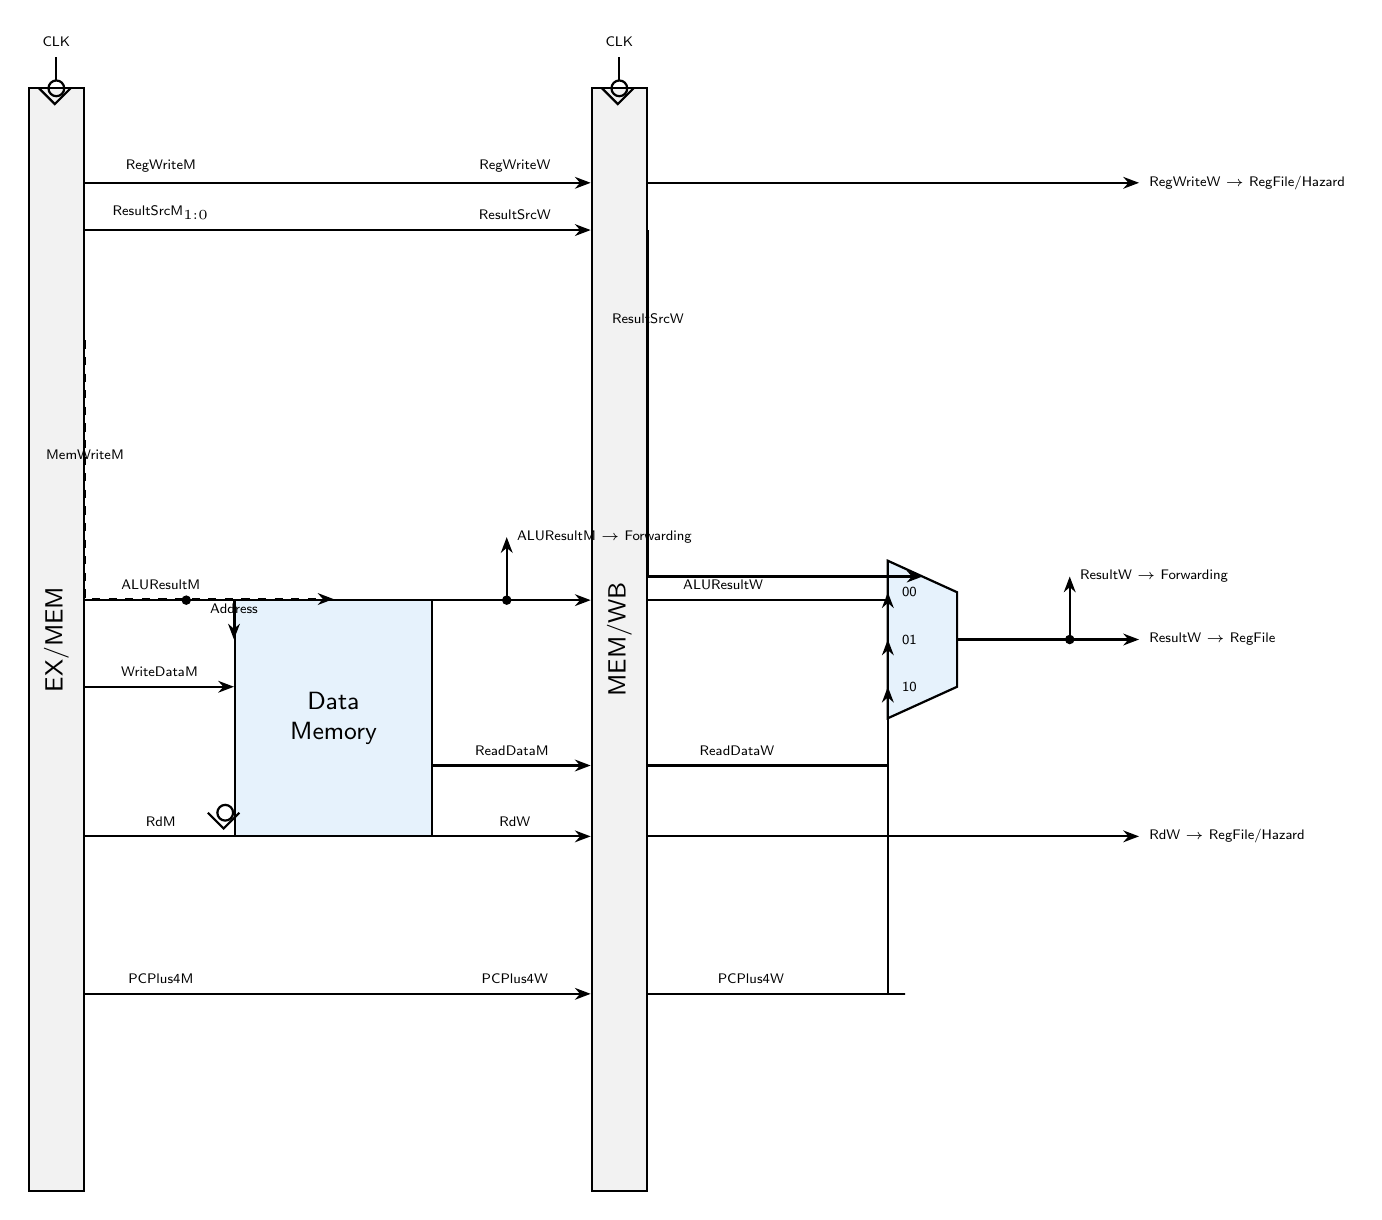
\begin{tikzpicture}[
  x=1.1cm, y=1.0cm,
  signal/.style={-{Stealth[length=2mm]}, thick, black},
  lbl/.style={font=\tiny\sffamily, text=black},
  lblcenter/.style={font=\small\sffamily, align=center},
]

% EX/MEM y MEM/WB Pipeline Registers
\node[draw, fill=gray!10, thick, minimum width=0.7cm, minimum height=14cm, font=\small\sffamily] (exmem_reg) at (0, 0) {\rotatebox{90}{EX/MEM}};
\node[draw, fill=gray!10, thick, minimum width=0.7cm, minimum height=14cm, font=\small\sffamily] (memwb_reg) at (6.5, 0) {\rotatebox{90}{MEM/WB}};

% Clocks
\draw[thick] (0.0, 7.0) circle (1mm);
\draw[thick] (0.0, 7.1) -- ++(0, 3mm) node[above, font=\tiny\sffamily] {CLK};
\draw[thick] (-0.2, 7.0) -- ++(2mm, -2mm) -- ++(2mm, 2mm);

\draw[thick] (6.5, 7.0) circle (1mm);
\draw[thick] (6.5, 7.1) -- ++(0, 3mm) node[above, font=\tiny\sffamily] {CLK};
\draw[thick] (6.3, 7.0) -- ++(2mm, -2mm) -- ++(2mm, 2mm);

% Componentes
\node[box, minimum height=3.0cm, minimum width=2.5cm, font=\small\sffamily, align=center] (dmem) at (3.2, -1.0) {Data\\Memory};
\draw[thick] (1.95, -2.2) circle (1mm);
\draw[thick] (1.75, -2.2) -- ++(2mm, -2mm) -- ++(2mm, 2mm); % clk pin

\drawmuxthree{10.0}{0.0}{muxR}{}

% Control signals straight passing
\draw[signal] (exmem_reg.east |- {0, 5.8}) -- (memwb_reg.west |- {0, 5.8}) node[lbl, pos=0.15, above] {RegWriteM} node[lbl, pos=0.85, above] {RegWriteW};
\draw[signal] (exmem_reg.east |- {0, 5.2}) -- (memwb_reg.west |- {0, 5.2}) node[lbl, pos=0.15, above] {ResultSrcM$_{1:0}$} node[lbl, pos=0.85, above] {ResultSrcW};

% Data Memory Write Enable control line (dashed)
\draw[signal, dashed] (exmem_reg.east |- {0, 3.8}) |- (dmem.north) node[lbl, pos=0.25, above] {MemWriteM};

% ALUResultM to MEM/WB and dmem address
\draw[signal] (exmem_reg.east |- {0, 0.5}) -- (memwb_reg.west |- {0, 0.5}) node[lbl, pos=0.15, above] {ALUResultM};
\draw[fill=black] (1.5, 0.5) circle (1.5pt);
\draw[signal] (1.5, 0.5) -| (dmem.west |- {0, 0.0}) node[lbl, pos=0.8, above] {Address};

\draw[signal] (exmem_reg.east |- {0, -0.6}) -- (dmem.west |- {0,-0.6}) node[lbl, midway, above] {WriteDataM};

% ReadData to MEM/WB
\draw[signal] (dmem.east |- {0, -1.6}) -- (memwb_reg.west |- {0,-1.6}) node[lbl, midway, above] {ReadDataM};

% Passing signals RdM, PCPlus4M
\draw[signal] (exmem_reg.east |- {0, -2.5}) -- (memwb_reg.west |- {0, -2.5}) node[lbl, pos=0.15, above] {RdM} node[lbl, pos=0.85, above] {RdW};
\draw[signal] (exmem_reg.east |- {0, -4.5}) -- (memwb_reg.west |- {0, -4.5}) node[lbl, pos=0.15, above] {PCPlus4M} node[lbl, pos=0.85, above] {PCPlus4W};

% From MEM/WB to Writeback MUX and beyond
\draw[signal] (memwb_reg.east |- {0, 0.5}) -- (9.0, 0.5) node[lbl, pos=0.4, above] {ALUResultW} -| (muxR_in0);
\draw[signal] (memwb_reg.east |- {0, -1.6}) -- (9.4, -1.6) node[lbl, pos=0.4, above] {ReadDataW} -| (muxR_in1);
\draw[signal] (memwb_reg.east |- {0, -4.5}) -- (9.8, -4.5) node[lbl, pos=0.4, above] {PCPlus4W} -| (muxR_in2);

% ResultSrcW selector
\draw[signal] (memwb_reg.east |- {0, 5.2}) |- (muxR_sel) node[lbl, pos=0.15, above] {ResultSrcW};

% Signals passing out to top/right
\draw[signal] (memwb_reg.east |- {0, 5.8}) -- (12.5, 5.8) node[right, lbl] {RegWriteW $\rightarrow$ RegFile/Hazard};
\draw[signal] (memwb_reg.east |- {0, -2.5}) -- (12.5, -2.5) node[right, lbl] {RdW $\rightarrow$ RegFile/Hazard};
\draw[signal] (muxR_out) -- (12.5, 0.0) node[right, lbl] {ResultW $\rightarrow$ RegFile};

% Forwarding branches tap-offs (represented as outputs)
\draw[fill=black] (5.2, 0.5) circle (1.5pt);
\draw[signal] (5.2, 0.5) -- (5.2, 1.3) node[right, lbl] {ALUResultM $\rightarrow$ Forwarding};

\draw[fill=black] (11.7, 0.0) circle (1.5pt);
\draw[signal] (11.7, 0.0) -- (11.7, 0.8) node[right, lbl] {ResultW $\rightarrow$ Forwarding};

\end{tikzpicture}
\end{document}
